\section{Organisation of the repository}

	\begin{minipage}{0.65\linewidth}
		For the organisation of the repository, we created several directories (Figure \ref{tree}):
		\begin{enumerate}[label=\textbullet]
			\item \textbf{src :} In this directory there is all the source code of the project. We have a first \textit{python} subdirectory which contains the python codes for the data assimilation and parareal parts, these files were created during the M1 project. Then we have a second subdirectory \textit{cpp} which contains the C++ codes of the same 2 parts.
			\item \textbf{examples :} Here there are examples of how to use python and C++ codes.
			\item \textbf{tests :} In this directory there are python and C++ tests of the code. For python tests we will use the pytest tool and for C++ we will use ctest (see Section \ref{compile}).
			\item \textbf{docs :} This directory gathers all the files that are used to generate the documentation of the project (see section \ref{doc}). The \textit{sphinx} and \textit{doxygen} directories enable respectively to document the python code and the C++ code (thanks to the sphinx~\cite{sphinx_doc} and doxygen~\cite{doxygen_doc} tools). The \textit{antora} directory contains some explanations of the project which are accessible online (the antora~\cite{antora_doc} tool was used). For example it explains : the differential equations concerned by this project, the data assimilation methods, the parareal method... The documentations generated by the previous tools are available directly in the GitHub repository via a Continuous Integration (CI) that has been set up (see section \ref{ci}).
			The directories \textit{gantt}, \textit{meeting}, \textit{presentation} and \textit{report} contain all the latex files and images used for the presentations and reports requested in the context of the internship.
			\item \textbf{cmake/build :} The directory \textit{cmake} contains cmake configuration files which are used for the compilation of the C++ project (see Section \ref{compile}). The directory \textit{build} contains all the files generated by the compilation of the C++ code.
		\end{enumerate}
	\end{minipage} \qquad
	\begin{minipage}{0.33\linewidth}
		\begin{figure}[H]
			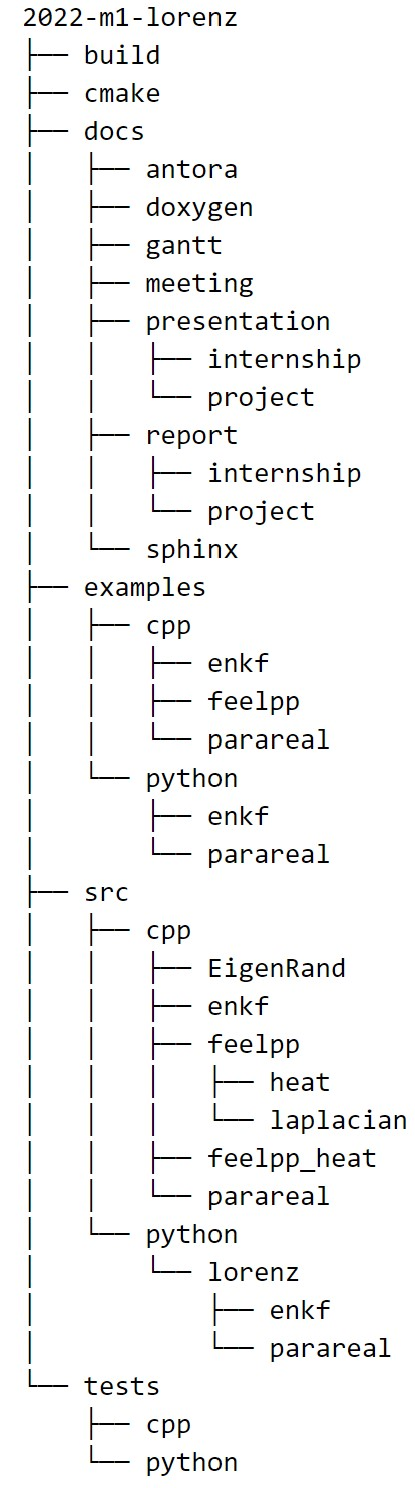
\includegraphics[width=\textwidth]{"images/appendix/tree.jpg"}
			\caption{Repository tree}
			\label{tree}
		\end{figure}
		%\lstinputlisting[language={},inputencoding=utf8]{tree.txt}
	\end{minipage}

\newpage

\section{Compile and test}
\label{compile}

	

\newpage

\section{Documentation}
\label{doc}

\section{Github actions}
\label{ci}